\documentclass[a4paper,norsk, 10pt]{article}
\usepackage[utf8]{inputenc}
\usepackage{verbatim}
\usepackage{listings}
\usepackage{graphicx}
\usepackage[norsk]{babel}
\usepackage{a4wide}
\usepackage{color}
\usepackage{amsmath}
\usepackage{float}
\usepackage{amssymb}
\usepackage[dvips]{epsfig}
\usepackage[toc,page]{appendix}
\usepackage[T1]{fontenc}
\usepackage{cite} % [2,3,4] --> [2--4]
\usepackage{shadow}
\usepackage{hyperref}
\usepackage{titling}
\usepackage{marvosym }
\usepackage{subcaption}
\usepackage[noabbrev]{cleveref}
\usepackage{cite}


\setlength{\droptitle}{-10em}   % This is your set screw

\setcounter{tocdepth}{2}

\lstset{language=c++}
\lstset{alsolanguage=[90]Fortran}
\lstset{alsolanguage=Python}
\lstset{basicstyle=\small}
\lstset{backgroundcolor=\color{white}}
\lstset{frame=single}
\lstset{stringstyle=\ttfamily}
\lstset{keywordstyle=\color{red}\bfseries}
\lstset{commentstyle=\itshape\color{blue}}
\lstset{showspaces=false}
\lstset{showstringspaces=false}
\lstset{showtabs=false}
\lstset{breaklines}
\title{FYS2140, Oblig 1}
\author{Daniel Heinesen, daniehei}
\begin{document}
\maketitle

\section*{2.4)}


\subsubsection*{d)}\label{subsec::overforingAvAllEnergi}
For å finne ut om et foton kan overføre all energien sin til et elektron, må vi se på bevaring av bevelgelsesmengde og energi. Vi velger et referansepunkt hvor elektronet ikke har noe bevegelsesmengde før sammenstøtet. Fotonet forvinner også etter sammenstøtet og har da verken energi eller bevegelsesmengde. Vi får da at bevegelsesmengdene er:

$$
p_e = p_e
$$
$$
p_{\gamma} = \frac{h}{\lambda}
$$

Og energiene:

$$
E_{e,before} = m_ec^2
$$

$$
E_e = \sqrt{p_e^2c^2 + m_e^2c^4}
$$
$$
E_{\gamma} = \frac{hc}{\lambda}
$$

Bruker vi bevaring og setter inn utrykket for $p_e$ inn i $E_e$ får vi at:

$$
m_ec^2 + \frac{hc}{\lambda} = \sqrt{p_e^2c^2 + m_e^2c^4} = \sqrt{(\frac{h}{\lambda})^2c^2 + m_e^2c^4}
$$

Løser vi opp kvadratroten får vi at

$$
m_e^2c^4 +2\frac{m_ehc^3}{\lambda} + \frac{h^2c^2}{\lambda^2} = \frac{h^2c^2}{\lambda^2} + m_e^2c^4
$$

$$
\Rightarrow 2\frac{m_ehc^3}{\lambda} = 0
$$

Men vi vet at verken $m_e$,$\lambda$ eller $c$ er $0$, og derfor er $2\frac{m_ehc^3}{\lambda} \ne 0$. Vi har derfor en motsigelse, hvilket betyr at fotonet ikke kan gi all energien sin til elektronet.

\section*{2.8)}

\subsection*{a)}

\begin{figure}[H]
\centering
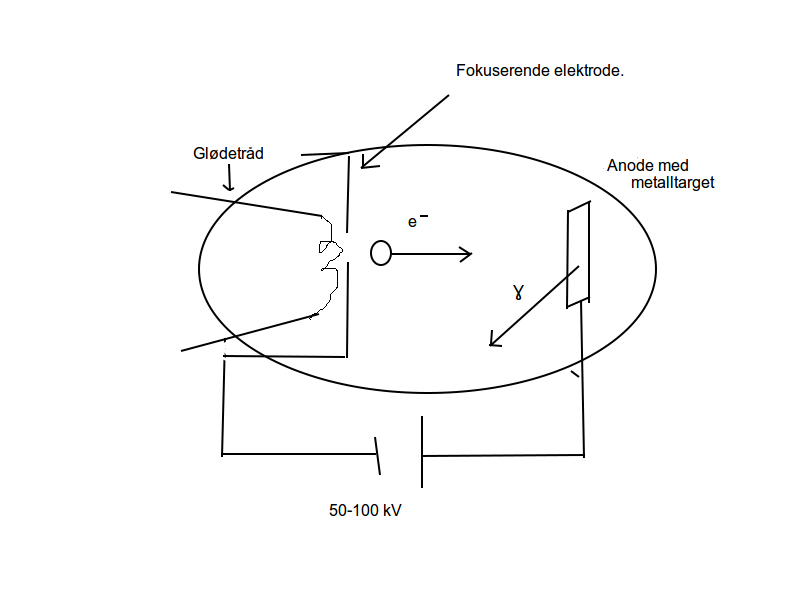
\includegraphics[scale=.4]{rontgen.png}
\caption{Skimatisk tegning av en røtgenrør.}\label{img::rontgenror}
\end{figure}

I figuren over \ref{img::rontgenror} ser vi en enkel tegning av et røtgenrør. Elektroner blir laget av glødetråden og akselereres så mot og igjennom den fokuserende elektroden. Spenningsforskjellen mellom denne elektroden og anoden (rundt 50-100 kV) på forsetter og akselerere elektroden før det tilslutt kræsjer inn i metalltargeten. Inne i metallet vil atomene bremse opp elektronet. Den energien som tapes av elektronet vil gå over i stråling, \textit{Bremsstrahlung}. For systemer som dette vil stråling være i form av røntgenstråling ($\lambda = 0.01 - 10$ nm).

\subsection*{b)}
Fra kompendiumet finner vi at $\lambda_{min}$ ved

$$
\lambda_{min}  = \frac{hc}{eV_R}
$$

Om elektronet har kinetisk energi $K_e = 10000$ eV vil dette gi en minste bølgelengde på:

$$
\lambda_{min} =  \frac{hc}{10000 \mathrm{eV}} = 1.24 \cdot 10^{-10} \mathrm{m}
$$

\subsection*{c)}
Når fotonet treffer krystallen vil en del av lyset reflekteres fra overflaten på krystallen. Noe av lyset vil også igjennom og treffe laget under(eller under der igjen) og reflekteres. Det lyset som reflekteres av laget under vil ha en lengre vei å gå enn det lyset som ble reflektert av overflaten. Dette vil føre til en faseforskyvning. Om avstanden lyset må reise mellom lagene ikke er $n\lambda$ vil fasene til lyset fra de forskjellige lagene ikke være like, og man får destruktiv interferens. Er denne avstanden derimot $n\lambda$ vil fasene være like og lysstrålen vil forsette med samme stryrke men nå i en annen vinkel(refleksjonen). Formelen som beskriver dette (når man får en refleksjon) er:

$$
n\lambda = 2d\sin(\theta)
$$

Vi vet at $\lambda = 1$ nm, $\theta = 45^{\circ}$, og vi er bare interessert i det øverste laget, så vi sier at $n = 1$

$$
d = \frac{\lambda}{2\sin(\theta)} = 0.71 nm
$$

\section*{d)}
Vi ønsker å finne minst mulig fotonenergi $E_{\nu}$ for å få pardannelse. Et elektronpar har minst energi når det står i ro. Den har da ingen bevegelsesmengde, $p_e = 0$. For å finne energien setter vi opp energibevaring. Energien til fotonet $E_{\nu}$, må være like energien til elektronparret etter dannelsen. Vi antar også at fotonet blir borte etter dannelsen. Vi har da at

$$
E_{\nu} = 2\sqrt{p_c^2c^2 + m_e^2c^4}
$$

Men vi vet at elektronet ikke har noe bevegelsesmengde, så vi sitter da igjen med:

$$
E_{\nu} = 2m_ec^2
$$

Med andre ord hvileenergien til de 2 elektronene. Vi har et problem, og det er at selv om energi er bevart, så er ikke bevegelses mengde det. Fotonet hadde trossalt bevegelsesmengde før dannelsen, men det er borte etter, og elektronene står stille. En slik prosess kan derfor bare skje nær en atomkjerne, da det er denne som tar over all bevegelsesmengden til fotonet. Om dette ikke er tilfellet vil ikke denne prosessen være mulig(som sett i oppgave 2.8d \ref{subsec::overforingAvAllEnergi}). Kjernen må også ta over litt av energien til fotonet med bevegelsesmengden. Men vi ønsker her en ideel situasjon, så vi antar at den ikke får noe av energien.

\section*{2.9)}

\subsection*{a)}
Interaksjonen mellom fotonet og elektronet kan sees i figuren under\ref{fig::photonElectronCollision}.

\begin{figure}[H]
\centering
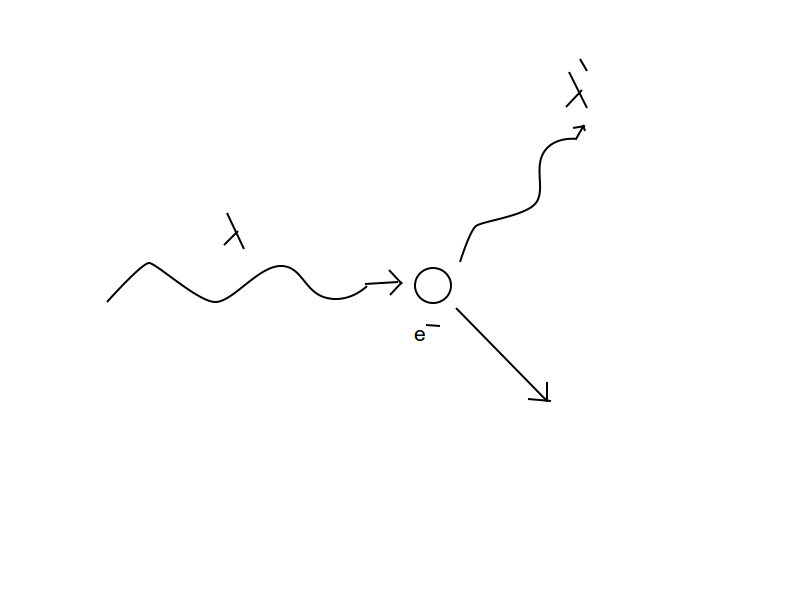
\includegraphics[scale=.3]{comptonLambda.png}
\caption{Figuren viser kollisjonen mellom et foton og et elektron.}\label{fig::photonElectronCollision}
\end{figure}

I en slik kollisjon må både energy og bevegelsesmengde må være bevart. Energiene er gitt som

$$
E_{\gamma} = \frac{hc}{\lambda}
$$
$$
E_e = \sqrt{p_2^2c^2 + m_e^2c^4}
$$

Før kollisjonen står elektronet stille nær kjernen og har bare hvileenergi. Etter har det både en energi og bevegelsesmengde. Før kollisjonen har fotonet bølgelengde $\lambda$ og etter kollisjonen har det $\lambda'$.

Vi skal anta senere at bevegelsesmengden til fotonet er gitt ved

$$
p_{\gamma} = \frac{h}{\lambda}
$$

Men inntil videre skal vi la den stå som ukjent. Før kollisjonen har elektronen ingen bevegelsesmengde, og etter kollisjonen har den en ukjent bevegelsesmengde. Vi kan regne ut denne bevegelesmengden ved å se på bevaring av energien:

$$
m_ec^2 + \frac{hc}{\lambda} = \sqrt{p_2^2c^2 + m_e^2c^4} + \frac{hc}{\lambda'}
$$

Hvilket gir at:

\begin{equation}
p_e^2c^2 = \big(m_ec^2 + \frac{hc}{\Delta \lambda} \big)^2 - (m_ec^2)^2
\end{equation}\label{eq::p2c2}

Hvor $\Delta \lambda = \lambda - \lambda'$.\\

Vi bruker så bevaring av bevegelsesmengde:

$$
\vec{p_{\gamma}} = \vec{p_e} + \vec{p_{\gamma'}} \Leftrightarrow \vec{p_{e}} = \vec{p_{\gamma}} - \vec{p_{\gamma'}}
$$

Hvor $\vec{p_{\gamma'}}$ er bevegelsesmengden til fotonet etter kollisjonen. Vi finner så at:

$$
(p_e)^2 = \vec{p_e} \cdot \vec{p_e} = p_{\gamma'}^2 + p_{\gamma}^2 - 2p_{\gamma}p_{\gamma'}\cos(\theta)
$$

Vi kan nå bruke antagelsen om bevegelsesmengden til fotonet, og i tillegg ganger vi begge siden med $c^2$

\begin{equation}
(p_ec)^2 = \left(\frac{hc}{\lambda}\right)^2 + \left(\frac{hc}{\lambda'}\right)^2 - 2\left(\frac{hc}{\lambda \lambda'}\right)\cos(\theta)
\end{equation}\label{eq::p2c22}

Vi har nå 2 uttykk vi kan sette like hverandre:

$$
\left(\frac{hc}{\lambda}\right)^2 + \left(\frac{hc}{\lambda'}\right)^2 - 2\left(\frac{hc}{\lambda \lambda'}\right)\cos(\theta) = \big(m_ec^2 + \frac{hc}{\Delta \lambda} \big)^2 - (m_ec^2)^2
$$

Å løse dette for $\Delta \lambda$ er en ren algebraisk oppgave, og for mye å skrive i Latex. Men resultatet man får er Comptons formel:

\begin{equation}
\Delta \lambda = \frac{h}{m_ec}(1-\cos(\theta))
\end{equation}\label{eq::compton}


\subsection*{b)}

Etter en kollisjon må fotonet ha gitt noe av sin energi til elektronet. Energien til fotonet er gitt ved $E = \frac{hc}{\lambda}$. Siden både $h$ og $c$ er konstanter, så må en lavere energi bety en høyere bølgelengde $\lambda$.\\

Vi kan også se det fra Comptorn formelen \ref{eq::compton}. Siden $\cos\theta$ er mindre enn 1, blir $\Delta \lambda > 0$, hvilket betyr at $\lambda < \lambda'$.

\subsection*{c)}
Før kollisjonen har fotonet bevegelsesmengde $p_{\gamma} = \frac{h}{\lambda}$ og elektronet $p_e = - p_{\gamma}$. Etter kollosjonen har de $p_{\gamma}' = \frac{h}{\lambda'}$ og $p_e'$. Bruker vi bevaring av bevegelsesmengde finner vi at:

$$
p_{\gamma} + p_e = p_{\gamma} + (-p_{\gamma}) = 0 = p_e' + p_{\gamma}'
$$

$$
\Rightarrow p_e' = - p_{\gamma}' = -\frac{h}{\lambda'}
$$

Vi bruker så dette utrykket i energibevaring:

$$
E_e + E_{\gamma} = E_e' + E_{\gamma}'
$$
$$
\sqrt{p_e^2c^2 + m_e^2c^4} + \frac{hc}{\lambda} = \sqrt{p_e'^2c^2 + m_e^2c^4} + \frac{hc}{\lambda'}
$$

$$
\sqrt{\frac{h^2c^2}{\lambda^2} + m_e^2c^4} + \frac{hc}{\lambda} = \sqrt{\frac{h^2c^2}{\lambda'^2} + m_e^2c^4} + \frac{hc}{\lambda'}
$$

For at dette skal stemme må $\lambda = \lambda'$. M.a.o. er $\Delta \lambda = 0$

\subsection*{d)}
Se oppgave 2.4d \ref{subsec::overforingAvAllEnergi}


\end{document}


